\documentclass[10pt]{article}
\usepackage[a4paper, textwidth=16cm, textheight=24cm]{geometry}
\usepackage{ctex}
\usepackage{graphicx}
\usepackage{amsmath}
\usepackage{subfigure}

\title{\textbf{作业二~~基于 RPCA 的图像去噪实验报告}}
\author{刘行 PB22000150}
\date{\today}

\begin{document}
	\maketitle

	\section{实验原理}
		本实验基于\textbf{鲁棒主成分分析 (RPCA) }进行图像去噪. RPCA 假设一个观测矩阵 $A$ 由两部分组成:

		\begin{itemize}
			\item \textbf{低秩矩阵 $L$}: 表示主要的结构信息 (如图像的主体部分).
			\item \textbf{稀疏矩阵 $S$}: 表示异常值或噪声 (如图像中的损坏区域或遮挡物).
		\end{itemize}

		即:
		\begin{equation}
		A = L + S
		\end{equation}

		为了分解$A$, 采用如下优化问题:
		\begin{equation}
			\min_{L, S} \|L\|_* + \lambda \|S\|_1, \quad \text{s.t.} \quad A = L + S
		\end{equation}
		其中:

		\begin{itemize}
			\item $\|L\|_*$ 为核范数, 即$L$的奇异值之和, 鼓励$L$具有低秩结构.
			\item $\|S\|_1$ 为L1范数, 即矩阵元素绝对值之和, 鼓励$S$具有稀疏性.
			\item $\lambda$ 是一个超参数, 用于平衡低秩部分和稀疏部分.
		\end{itemize}

		优化问题可通过\textbf{增强拉格朗日乘子法 (ALM) }求解.

	\section{代码分析}

		本实验实现了MATLAB GUI界面, 支持图像加载、去噪处理和结果保存. 主要代码结构如下:

		\begin{itemize}
			\item \texttt{load\_image()}: 加载图像并显示.
			\item \texttt{run\_rpca()}: 执行RPCA去噪, 并显示低秩部分 (去噪图像) 和稀疏部分 (噪声).
			\item \texttt{save\_result()} 和 \texttt{save\_noise()}: 分别保存去噪后的图像和噪声部分.
		\end{itemize}

		在RPCA求解过程中, \texttt{rpca()} 函数使用\textbf{奇异值软阈值化}和\textbf{L1软阈值化}更新$L$和$S$. 此外, 我们将$\lambda$调整为$10/\max\left(m, n\right)$, 这样可以更好地控制稀疏矩阵$S$, 提高去噪效果. 事实上在实验过程中发现, 取 $\lambda = 1 / \max\left(m, n\right)$ 会使下面的第一个实验结果白色色块偏红.

	\section{操作说明}
		\begin{enumerate}
			\item 点击``Load Image''按钮加载测试图像.
			\item 点击``RPCA with each color''按钮进行图像去噪.
			\item 观察``Denoised Image''窗口 (去噪结果) 和``Noise Component''窗口 (噪声部分).
			\item 使用``Save Result''或``Save Noise''按钮保存图像.
		\end{enumerate}

	\section{实验结果}
		本实验采用两组图片进行测试, 每组包含原图、去噪图像和提取的噪声部分.

		\begin{figure}[htbp]
			\centering
			\subfigure[原始图像]{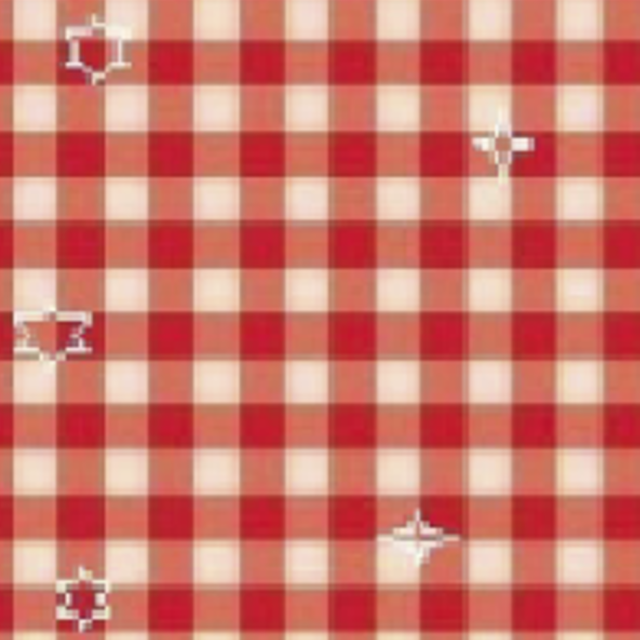
\includegraphics[width=0.3\textwidth]{figure/test_11.png}}
			\subfigure[去噪图像]{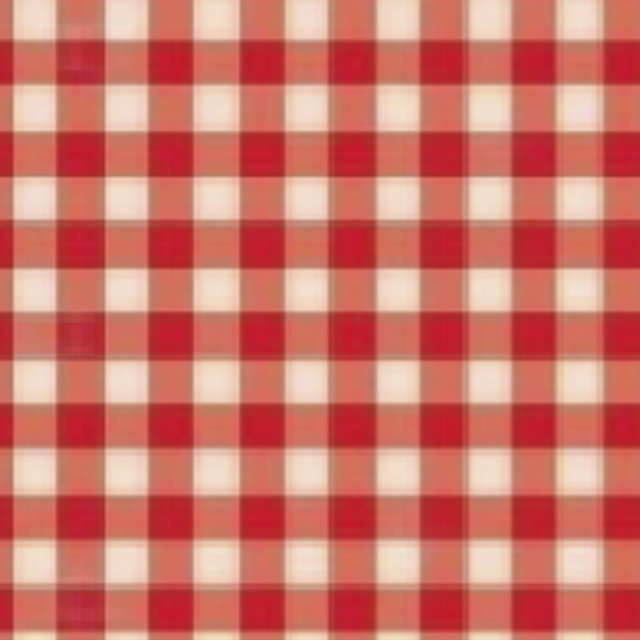
\includegraphics[width=0.3\textwidth]{figure/test_12.png}}
			\subfigure[噪声部分]{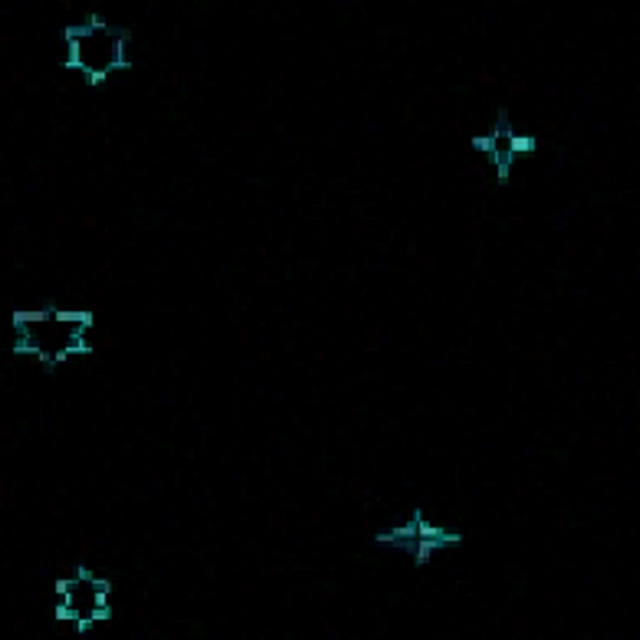
\includegraphics[width=0.3\textwidth]{figure/test_13.png}}
			\caption{第一组实验结果}
		\end{figure}

		\begin{figure}[htbp]
			\centering
			\subfigure[原始图像]{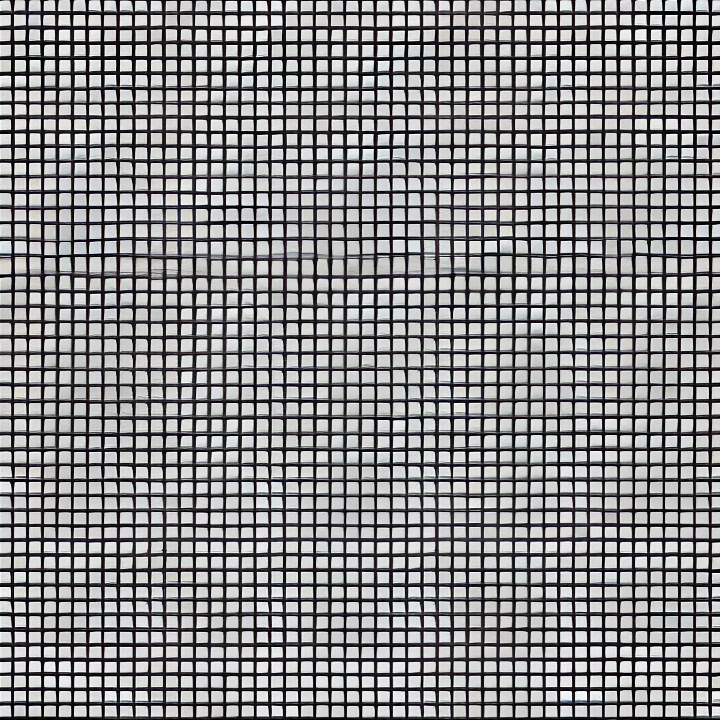
\includegraphics[width=0.3\textwidth]{figure/test_21.png}}
			\subfigure[去噪图像]{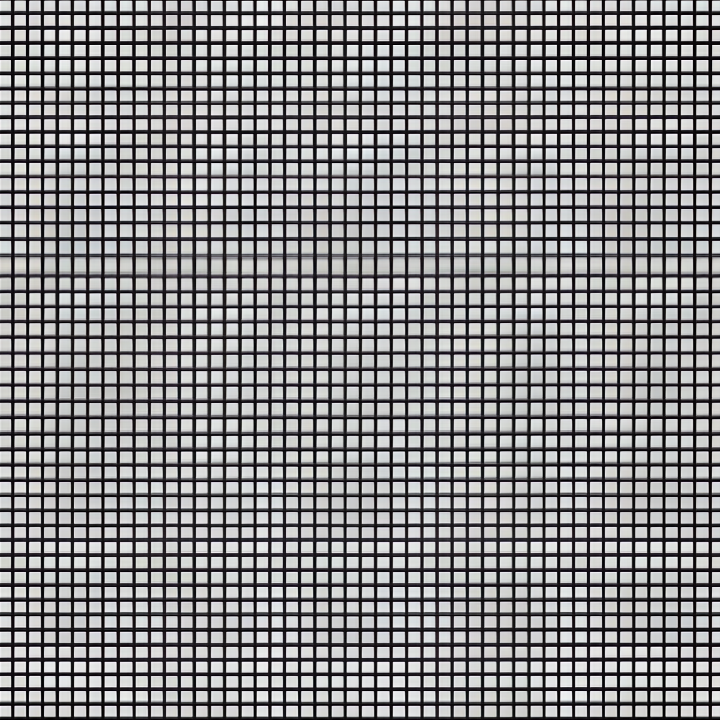
\includegraphics[width=0.3\textwidth]{figure/test_22.png}}
			\subfigure[噪声部分]{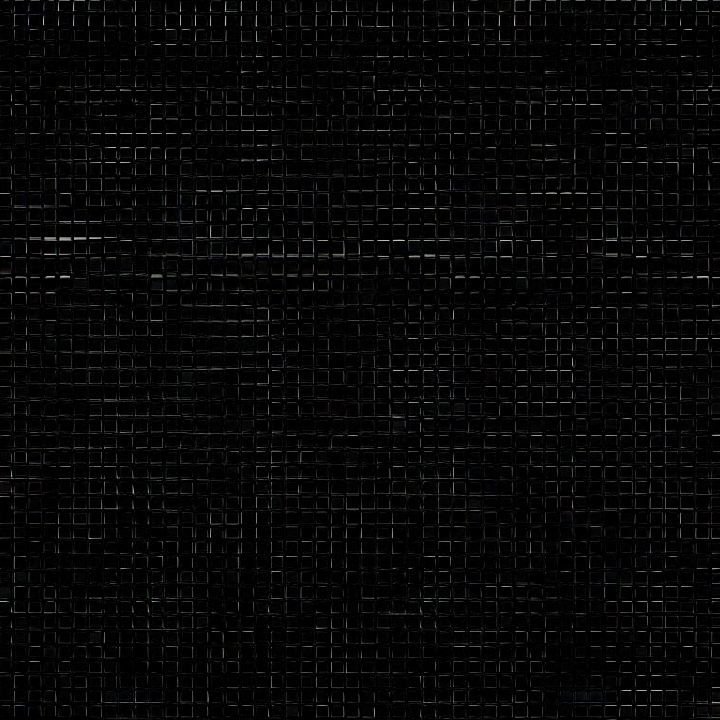
\includegraphics[width=0.3\textwidth]{figure/test_23.png}}
			\caption{第二组实验结果}
		\end{figure}

	\section{问题分析}
		实验结果表明, RPCA在去除随机噪声方面表现良好, 但对图像内容有一定限制:

		\begin{enumerate}
			\item \textbf{降噪后出现格状纹路}: 由于RPCA倾向于保留低秩信息, 对于原本没有网格结构的图像, 去噪后可能出现明显的格状纹路.
				\begin{figure}[htbp]
					\centering
					\subfigure[原始图像]{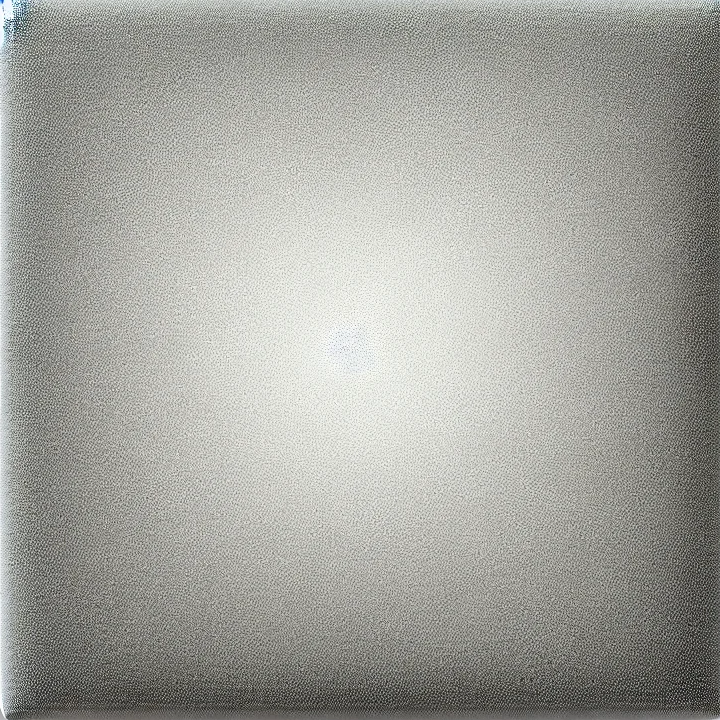
\includegraphics[width=0.3\textwidth]{figure/test_31.png}}
					\subfigure[去噪图像]{
\includegraphics[width=0.3\textwidth]{figure/test_32.png}}
					\subfigure[噪声部分]{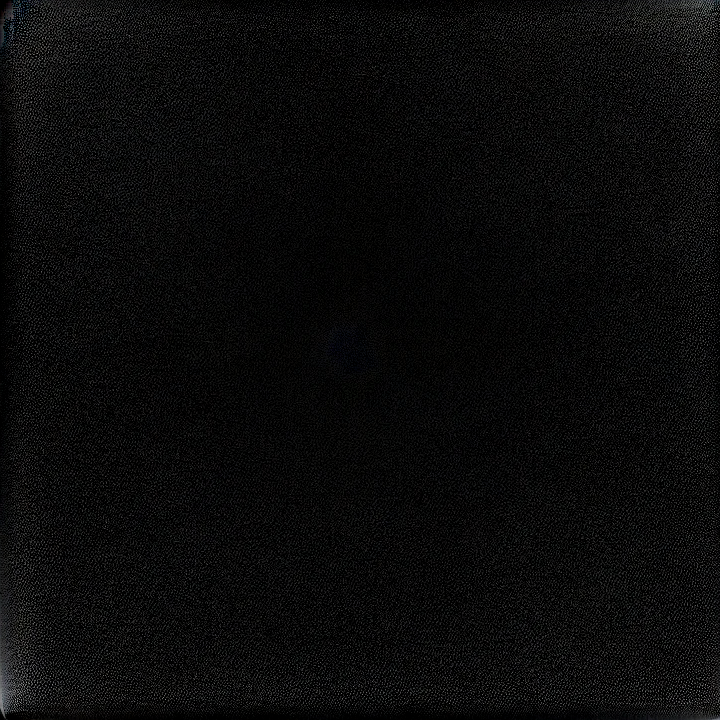
\includegraphics[width=0.3\textwidth]{figure/test_33.png}}
					\caption{网格结构图像实验结果}
				\end{figure}

			\item \textbf{仅对规则图案效果较好}: RPCA假设低秩结构, 因此对于纵横方向具有规则纹理的图像, 能够较好地去噪. 但对于复杂自然图像, 效果有限.
				\begin{figure}[htbp]
					\centering
					\subfigure[原始图像]{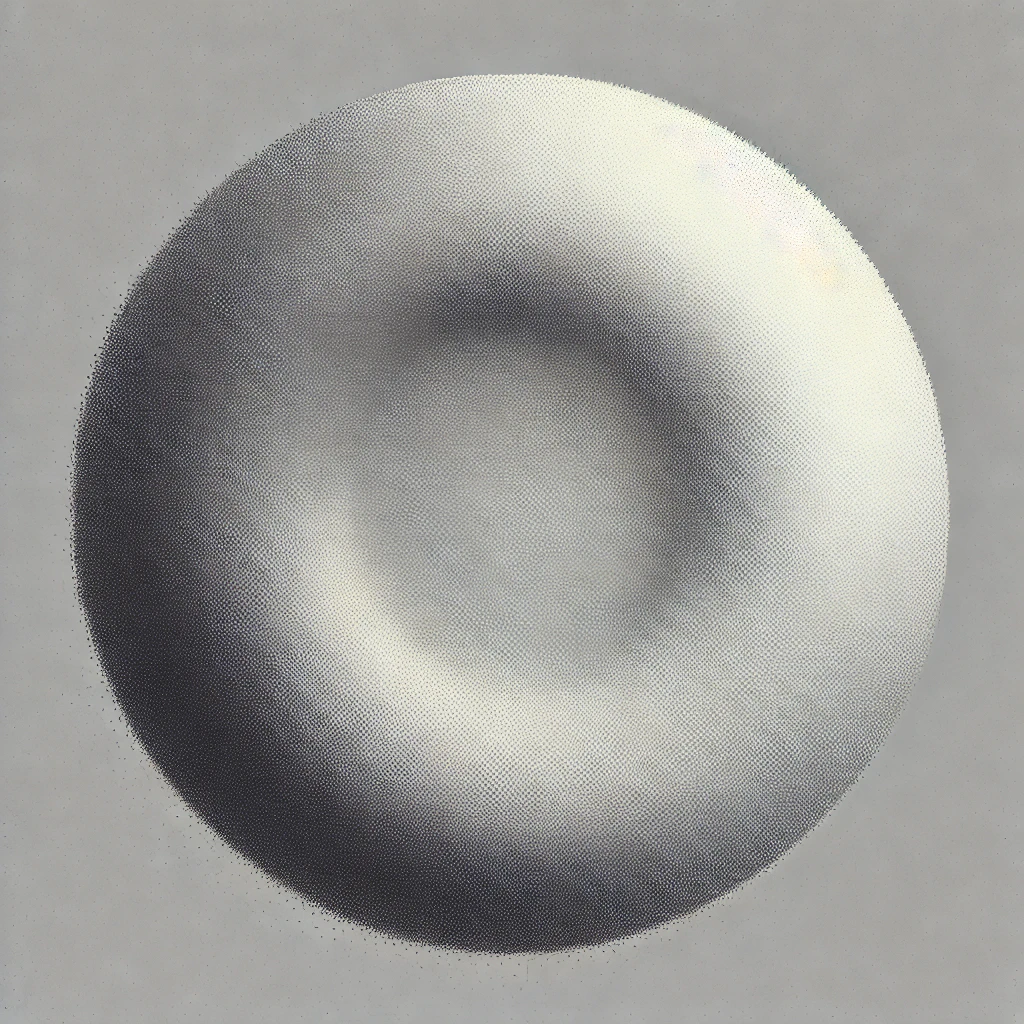
\includegraphics[width=0.3\textwidth]{figure/test_41.png}}
					\subfigure[去噪图像]{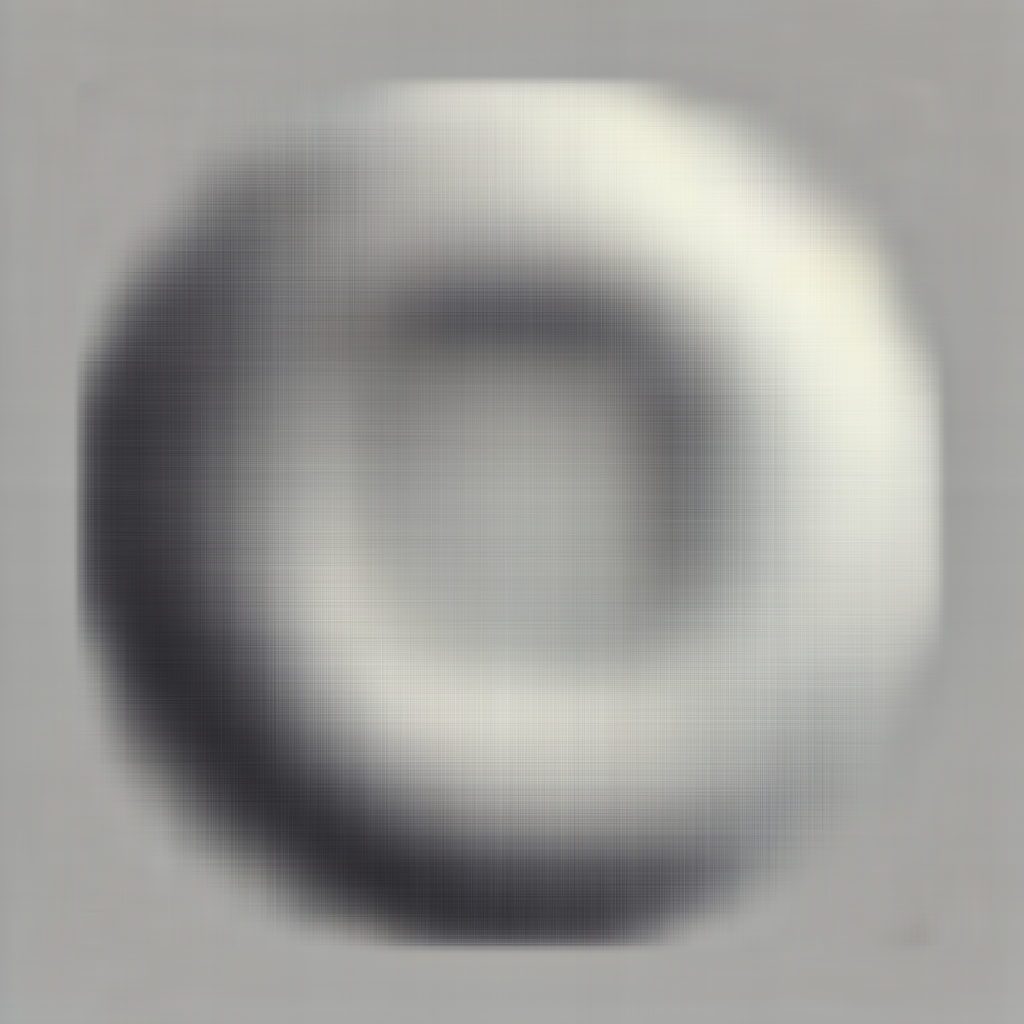
\includegraphics[width=0.3\textwidth]{figure/test_42.png}}
					\subfigure[噪声部分]{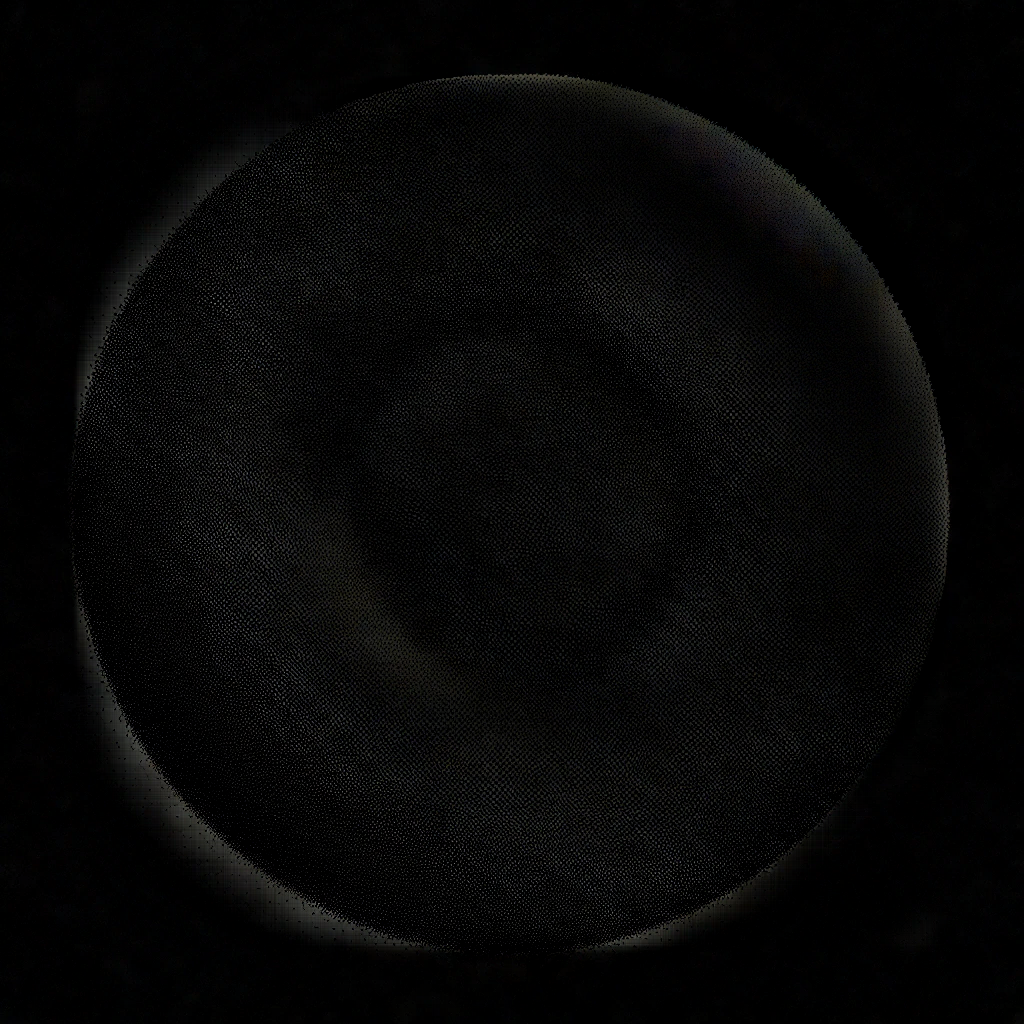
\includegraphics[width=0.3\textwidth]{figure/test_43.png}}
					\caption{规则图案实验结果}
				\end{figure}
		\end{enumerate}

		未来改进方向包括:

		\begin{itemize}
			\item 结合其他去噪方法, 如非局部均值滤波 (NLM).
			\item 研究不同的正则化策略, 提升对复杂图像的适应能力.
		\end{itemize}

\end{document}
